
\section{Problem Statement}\label{sec:adaptation:model}
For the sake of clarity, we will first state the task adaptation problem using notations from the previous chapter, and then highlight the connection between the concept learning problem and the latent task adaptation problem.

Formally, we define a classification \emph{task} to be a subset of all the possible object labels that are semantically related (such as all breeds of dogs in ImageNet). During training time, the computer is given all the training images from all these classes, and it will learn one single multi-class classifier. During testing time, a number of query images are randomly sampled from the labels belonging to a task, and the learning algorithm needs to give predictions on these images.

This scenario is much different from the conventional image classification problem setting, as being used in various benchmarks such as Caltech-101 \cite{fei2006one} and ILSVRC \cite{ilsvrc10}. Conventionally, we assume a set of mutually exclusive class labels to be presented during both training and testing time. From a probabilistic perspective, it means that the test images are assumed to be drawn i.i.d.\ from the same label distribution as the training images are. In our problem setting, testing images are mutually related since they together define the task. This makes more practical sense, since one may expect a computer agent to utilize its environment to preform better classification. For example, one could switch to classifying grocery items in a grocery store, and to classifying different animals during a zoo visit. It would be extremely unlikely (and not preferred) for an item in a grocery store to be a giraffe, given the context information.

As stated in the previous section, we are interested in the scenario when the task is \emph{latent}, \ie only implicitly specified by a set of test images. We introduce two key components for modeling the generative process of test images: a latent task space that defines possible tasks and their probability, and a procedure to sample images given a specific latent task. Specifically, we propose the graphical model in Figure \ref{fig:conceptgraph} which generates a set of $N$ test images when given $T$ possible tasks and $K$ object categories:
\begin{enumerate}
  \item Sample a latent task $h$ from the task priors $P(h)$ with hyperparameter $\balpha$;
  \item For the $N$ images:
    \begin{enumerate}
        \item Sample an object category $y_i$ from the conditional probability $P(y_i|h; \bbeta_{h})$;
        \item Sample an image from category $y_i$ with $P(x_i | y_i; \btheta_{y_i})$.
    \end{enumerate}
\end{enumerate}
where the parameters $\balpha, \bbeta, \btheta$ are defined as in the previous chapter.

\begin{figure}
  \centering
  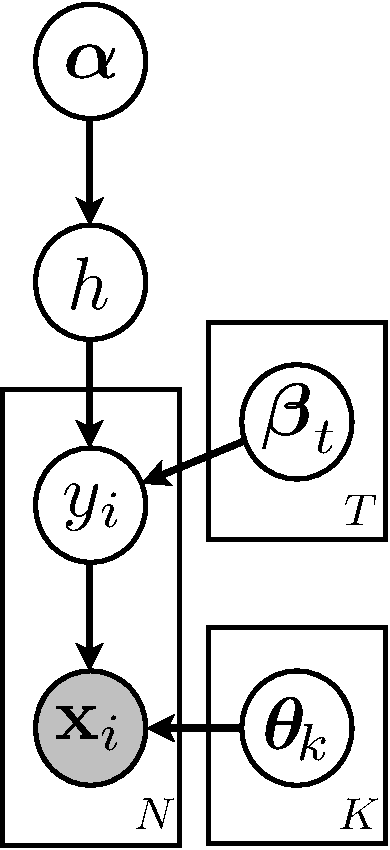
\includegraphics[width=0.15\textwidth]{figs/taskadaptation/our_model_vertical.pdf} \hspace{0.25in}%
  \caption{The generative model for the latent task and corresponding query images.}\label{fig:conceptgraph}
\end{figure}

A keen reader may have found the equivalence between a latent \emph{task} described here and a latent \emph{concept} described in the previous chapter. Indeed, they share much in common in the sense that both represent semantically related groups of objects in the real world. Thus, it is natural that one may consider classification in a gradual coarse-to-fine way, with each semantic group forming as a possible task, such as pet breeds of different brands of cars. This is the reason we do not distinguish these two terms, and consider latent concepts as latent tasks as well.

Admittedly, the definition of ``task context'' is much broader than merely groups of objects derived from a hierarchy. For example, another choice of defining tasks is to relate it to scenes - all objects in an office, or all objects that one may encounter in a street view. In these cases, a task may contain a set of objects that do not belong to, or at least are not well modeled by a taxonomical hierarchy. However, one may reasonably come up with such sets of tasks by looking into meta training data, most notably as co-occurrence of objects in an annotated database such as LabelMe \cite{russell2008labelme}. Thus, we will consider the formation of a latent task space an orthogonal problem, and leave it to future work.

The previous chapter gives the definition of the priors and conditionals, and for the sake of clarity, we will briefly review it here. The prior distribution $P(h)$ is modeled by an Erlang distribution with respect to the size $|h|$ of each latent task, defined as the number of leaf nodes in the subtree rooted at the task:
\begin{equation}
    P(h) = \alpha_h \propto (|h|/\sigma^2) \exp(-|h|/\sigma).
\end{equation}
We also choose the hyperparameter $\sigma$ so that it favors medium-sized tasks, as the last chapter did. The justification is that classification under medium-sized tasks usually correspond to fine-grained recognition problems, which is of particular interest in the literature: an agent that recognizes multiple species of dogs or multiple types of cars may be much more useful than an agent that coarsely classifies dogs vs cars.

Thee conditional probability $P(y_i | h)$ is defined using the strong sampling assumption and the size principle \cite{tenenbaum2001generalization}:
\begin{equation}
    P(y_i | h) = \beta_{hy_i} = \left\{\begin{array}{ll}
            1/|h|, & \text{if task } h \text{ contains leaf node label } y_i\\
                0, & \text{otherwise},
        \end{array}\right.
\end{equation}
where $|h|$ is the size of the task. The conditional probability of a specific image given a label is again defined in a mixture of generative and distriminative fashions, using the confusion matrix of the classifier as:
\begin{equation}
    P(\bx_i|y_i) \propto C_{y_if(\bx_i)},
\end{equation}
where $\bC$ is the confusion matrix of the classifier, $C_{ij}$ is the probability that an image from object class $i$ is predicted class $j$ by the classifier, and $f(\bx_i)$ is the classifier prediction
\begin{equation}
    f(\bx_i) = \argmax{j}\quad \btheta_j^\top \bx_i.
\end{equation}
We note again that the probability $P(\bx_i|y_i)$ defined above is a little abuse of terminology, as the partition function is not explicitly given. However, during inference this will only account for a constant bias in the overall likelihood, and will not change the final prediction.

\section{Linear Time MAP Inference}\label{sec:algo}
With the probabilistic model given in Figure \ref{fig:conceptgraph}, and given a set of query images to classify as $\mathcal{X} = \{\bx_1, \bx_2, \cdots, \bx_N\}$, we formally define the latent task adaptation problem as to jointly identify the hidden task $h$ and the hidden labels $\mathcal{Y} = \{y_1, y_2, \cdots, y_N\}$ that maximizes the posterior probability
\begin{equation}\label{eqn:MAP}
    (\hat{h}, \hat{\mathcal{Y}}) = \argmax{h, \mathcal{Y}} P(h, \mathcal{Y} | \mathcal{X}).
\end{equation}
We note that the task adaptation problem focuses on assigning actual labels to both the latent task and the latent labels, while the visual concept learning problem in the last chapter focuses more on generalization, and only provides probability that models the semantic closeness of new query images to the set of example images. This lead to the difference in the inference phase, while the generative model stays the same for both problems.

As most of the parameter estimation are similar to the previous chapter, we will focus on discussing the difference during the inference phase. Specifically, we will propose an efficient inference algorithm that allows one to perform both offline and online adaptation to the task context.

A conventional way to do probabilistic inference with nested latent variables is to use variational inference or Gibbs sampling, both of which find lower bounds of the posterior probability. This, however, may involve multiple iterations over the hidden variables and may be slow. We show that when the latent task space is organized in a DAG structure (as is the case in the ImageNet data), the exact maximum a posteriori (MAP) estimation (Eqn.\ (\ref{eqn:MAP})) could be found with an efficient dynamic programming algorithm that has complexity linear to the number of possible tasks.

We first note that the logarithm of posterior probability in Eqn.\ \ref{eqn:MAP} could be expanded as
\begin{equation}
\log P(h, \mathcal{Y} | \mathcal{X}) \propto \log\alpha_h + \sum\nolimits_{i=1}^{N}\log(\beta_{hy_i}C_{y_if(\bx_i)}).
\end{equation}
Notice that the size constraint defining the latent task space gives us
\begin{equation}
    \beta_{hy_i} = \frac{1}{|h|}I(y_i \in h),
\end{equation}
Eqn.\ \ref{eqn:MAP} could further be written as
\begin{equation*}
    \log\alpha_h - N \log|h| + \sum\nolimits_{i=1}^{n} (\log C_{y_if(\bx_i)} + \log I(y_i\!\in\!h)),
\end{equation*}
where one can observe that $h$ and $\mathcal{Y}$ decouples except for the $I(y_i\in h)$ term, which eliminates hypotheses that do not have $y_i$ by setting the log probability to negative infinity. As the latent tasks are organized as a tree-based hierarchy, we can define auxiliary functions
\begin{equation}
q_i(h) = \max_{\mathcal{Y}} \left[\log C_{y_if(\bx_i)} + \log I(y_i\in h)\right],
\end{equation}
which could be computed recursively as
\begin{equation}
q_i(h) = \max\nolimits_{\{h' \in child(h)\}} q_i(h'),
\end{equation}
where $child(h)$ is the set of children of $h$ in the tree. Finally, the latent task could be estimated as
\begin{equation}\label{eqn:taskargmax}
    \hat{h} = \argmax{h} \big[\log(\alpha_h) - N\log|h| + \gamma\sum\nolimits_{i=1}^{N} q_i(h)\big],
\end{equation}
and the corresponding $\hat{y}_i$s could be identified by taking the $\mathrm{argmax}$ of the corresponding $q_i(h)$.

We note that we added a hyperparameter $\gamma$ in the equation above. In practice, simply finding the MAP solution (using $\gamma=1$) often involves a task that is smaller than the ground truth, as there are two ways to explain the predicted labels: assuming correct prediction and a task of larger size, or assuming wrong prediction and a task of smaller size. The latter is preferred by the size principle, especially for classes with low classification accuracy. We found it beneficial to explicitly add a weight term that favors the classifier outputs using $\gamma>1$ learned on validation data.

In general, our dynamic programming method runs in $O(T\!Nb)$ time where $T$ is the number of tasks, $N$ is the number of query images, and $b$ is the branching factor of the tree (usually a small constant factor). This complexity is linear to the number of testing images and to the number of latent tasks, and is usually negligible compared to the basic classification algorithm, which runs $O(K\!N\!D)$ time where $K$ is the number of classes and $D$ is the feature dimension (usually very large).

%\subsection{Online Task Discovery and Classification}
Finally, one may prefer an online algorithm that could take new images as a stream, performing classification sequentially while discovering the latent task on the fly. We note that our method could be easily adapted to this end. Specifically, $q_i(h)$ serves as the sufficient statistics for the task discovery, and we only need to keep record of the accumulated auxiliary function values seen so far as 
\begin{equation}
    q_{:n}(h) = \sum\nolimits_{i=1}^{n-1} q_i(h)
\end{equation}
for the $n$-th image for each task candidate $h$. This allows us to perform online classification with $O(M)$ memory without storing the full history of images: when a new image $\bx_n$ arrives, one simply needs to compute $q_n(h)$ for all hypotheses, and compute its prediction by taking the argmax of $q_n(\hat{h_n})$ using the updated estimate of the task as
\begin{eqnarray}
    \hat{h_n} = \argmax{h} \big[\log(\alpha_h) - N\log|h| + \gamma(q_{:n}(h) + q_n(h))].
\end{eqnarray}

\section{Analyzing the Necessity of Task Adaptation}\label{sec:knowntask}
An important question to ask is whether we still want to do retraining instead of task adaptation, if one can afford retraining each task. In practice this is certainly impossible with potentially thousands of tasks, but it serves as a proof of concept whether task adaptation benefits overall classification.

To this end, we first analyze the benefits of retraining versus our adaptation method. Specifically, we sampled 5 subtrees from the ILSVRC hierarchy: {\texttt building}, {\texttt dogs}, {\texttt feline} (the superset of cats), {\texttt home appliance}, and {\texttt vehicle}, the subcategories of which are often of interest. Figure \ref{fig:tasks} visualizes the corresponding subtrees for dog, feline and vehicles respectively. Then, we explicitly trained classifiers on these three subtrees only, and compared the retrained accuracy against our adapted classifier with the given task. Since the task is known beforehand, during inference we will simply choose the prediction under the given task. We also tested two baselines: (1) the naive baseline that uses the raw 1000 class predictions, and (2) a forced choice baseline (FC), which simply selects the class under the task that has the largest output from the original classifiers. Table \ref{tab:knowntask} summarizes the performance of the algorithms.

It is worth pointing out that retraining the classifiers for the specific tasks does \emph{not} help improve the classification accuracy, although retraining requires additional nontrivial computation cost. In fact, it is always helpful to use out-of-task data to train a larger classifier and then take the subset with forced choice. One possible explanation is that this gives us more information about the general image statistics (similar to a better regularization term), as out-of-task images provide additional negative data during training. Our method further benefits from the statistics from all the classifiers (for in-task and out-of-task classes) in the proposed probabilistic framework. For example, when classifying different dogs, knowing the predicted score of e.g.\ fox and bears may still benefit the dog classification task under our framework, while the baseline algorithms fail to capture such information. As a result, the proposed algorithm achieves the best adapted accuracy in most cases (only slightly worse than the FC baseline on {\texttt vehicle}).

\begin{table}
    \centering
    \begin{tabular}{c|cccc}
        \hline \hline
        Task & Naive & Retraining & FC & Ours \\
        \hline
        {\texttt building} & 55.48 & 78.67 & 81.48 & {\bfseries 82.19} \\
        {\texttt dog} & 35.37 & 39.94 & 42.95 & {\bfseries 43.76}\\
        {\texttt feline} & 47.13 & 61.07 & 62.67 & {\bfseries 63.54}\\
        {\texttt home app} & 50.78 & 67.30 & 69.26 & {\bfseries 70.52} \\
        {\texttt vehicle} & 55.62 & 61.43 & {\bfseries 63.41} & 63.28\\
        \hline \hline
    \end{tabular}
    \caption{Classification accuracy on given tasks (subtrees) of the whole ILSVRC data. See subsection \ref{sec:knowntask} for details.}\label{tab:knowntask}
\end{table}

It is worth noting that such observation will be echoed when we move to the next chapter and analyze the transferability of deep features from state-of-the-art CNN models. This also hints the possibility to learn a general purpose image feature that adapts to multiple application purposes, which is one of the goal (and hope) of deep convolutional models.

\section{Experiments}
We conduct our experiment on the ILSVRC 2010 dataset \cite{ilsvrc}, where both validation and test data are available. To make sure we do not peek into the test images, all hyperparameters and classifiers are learned and validated on the training and validation data.

Also, we note that more comprehensive features and better classification pipelines may lead to better 1-vs-all accuracy on ImageNet, but it is not the main goal of the paper, as we focus on the adaptation on top of the base classifiers. Recent efforts on learning better classifiers, such as the ones presented in \cite{sanchez2011high,krizhevsky2012imagenet} could be seamlessly incorporated into our learning framework for general performance increases, and the next chapter will talk about a specific framework that enables on to do so in future research.

\subsection{Joint Task Discovery and Classification}

\begin{figure}
    \centering
    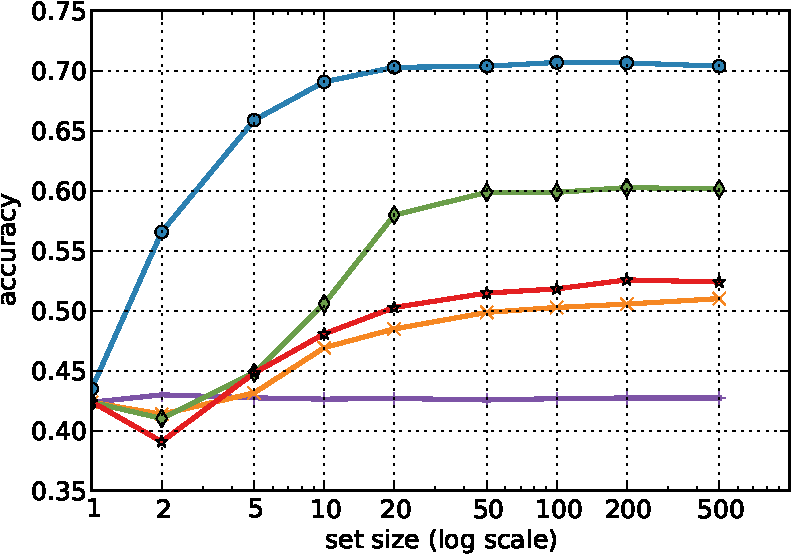
\includegraphics[width=0.45\textwidth]{figs/taskadaptation/offline_accuracy.pdf}%
    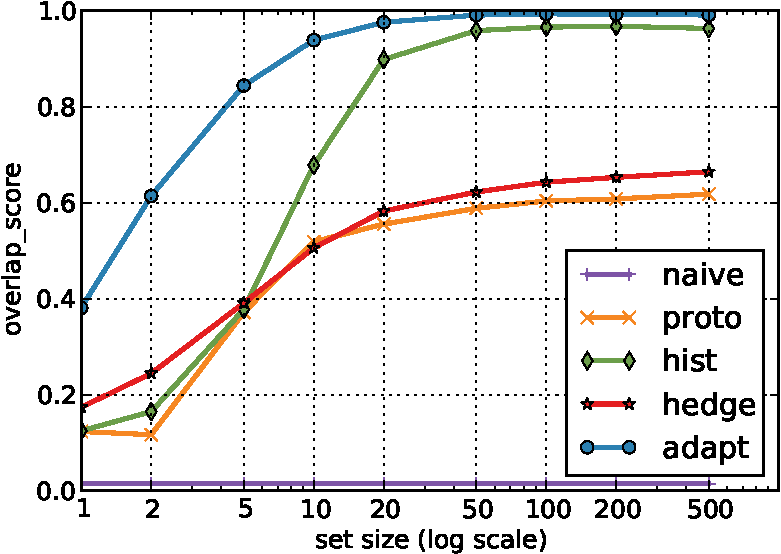
\includegraphics[width=0.45\textwidth]{figs/taskadaptation/offline_overlap_score.pdf}
    \caption{Classification accuracy (left) and the task overlap score (right) with different query set sizes for our method and the baselines.}\label{fig:jointclassify}
\end{figure}

\definecolor{naive}{rgb}{0.491, 0.331, 0.651}
\definecolor{proto}{rgb}{0.967, 0.530, 0.135}
\definecolor{hist}{rgb}{0.418, 0.621, 0.292}
\definecolor{hedge}{rgb}{0.894, 0.122, 0.129}
\definecolor{adapt}{rgb}{0.167, 0.502, 0.693}
\begin{sidewaysfigure}
    \centering
    \setlength\fboxsep{1.5pt}
    \setlength\fboxrule{0pt}
    \small
    \newcommand{\testim}[1]{\fbox{\begin{minipage}[c]{0.095\textwidth}\includegraphics[width=1.\textwidth,height=1.\textwidth]{figs/taskadaptation/thumbnails_sub/#1.JPEG}\end{minipage}}}
    \newcommand{\tasks}[5]{\multirow{4}{*}{\parbox{0.12\textwidth}{%
                \textcolor{naive}{#1}\\%
                \textcolor{proto}{#2}\\%
                \textcolor{hist}{#3}\\%
                \textcolor{hedge}{#4}\\%
                \textcolor{adapt}{#5}\\%
    }}}
    \newcommand{\task}[1]{\parbox{0.085\textwidth}{\raggedleft Task:\\#1}}
    \begin{tabular}{r|ccccc|c}
        \hline\hline
        \task{{\bfseries kitchen app}} & \testim{102835} & \testim{19992} & \testim{89217} & \testim{32216} & \testim{123376} & \tasks{entity}{artifact}{artifact}{goods}{kitchen app}\\
        Label & ice maker & espresso maker & primus stove & Dutch oven & ice maker & \\
         Ours & electric range & espresso maker & primus stove & Dutch oven & ice maker & \\
     Baseline & bookcase & web site & carpenter's kit & snail & scanner & \\
        \hline\hline
        \task{{\bfseries toiletry}} & \testim{100057} & \testim{40023} & \testim{78466} & \testim{48008} & \testim{59007} & \tasks{entity}{entity}{entity}{instrumentality}{toiletry}\\
        Label & lipstick & face powder & nail polish & lotion & hair spray & \\
         Ours & lipstick & face powder & nail polish & lotion & hair spray & \\
     Baseline & toothbrush & dune & bath towel & vending machine & military uniform & \\
        \hline\hline
        \task{{\bfseries wood- wind}} & \testim{125599} & \testim{11587} & \testim{146326} & \testim{10043} & \testim{4491} & \tasks{entity}{artifact}{artifact}{device}{reed}\\
        Label & bassoon & flute & sax & oboe & sax & \\
         Ours & bassoon & bassoon & sax & oboe & sax & \\
     Baseline & harp & prison & sax & fountain pen & turban & \\
        \hline\hline
        \task{{\bfseries game}} & \testim{19441} & \testim{124828} & \testim{64107} & \testim{109738} & \testim{139256} & \tasks{entity}{living thing}{entity}{chordate}{game}\\
        Label & ptarmigan & partridge & pheasant & black grouse & quail & \\
         Ours & ptarmigan & partridge & pheasant & black grouse & black grouse & \\
     Baseline & giant panda & orchid & Komodo dragon & Border collie & Newfoundland & \\
        \hline\hline
    \end{tabular}
    \caption{Exemplar classification results where incorrect labels are predicted by the base classifiers, but are corrected by our method that benefits from identifying the latent task. Each row shows 5 images from a latent task, and on the right we give the predicted task by different algorithms, ordered and colored as \textcolor{naive}{naive}, \textcolor{proto}{proto}, \textcolor{hist}{hist}, \textcolor{hedge}{hedge}, and \textcolor{adapt}{adapt}. The ground truth label, our prediction and the original classifier's output are provided for each image.}
\end{sidewaysfigure}

We analyze the performance when we have the classifier trained on the whole ILSVRC data, and adapt it to an unknown task that is defined by a set of query images. The forced choice option is not available in this case as we do not know the latent task beforehand, and one has to use the semantic relationships between the query images to infer the latent task.

To sample the latent tasks, we used the Erlang prior defined in Section \ref{sec:adaptation:model} from the ImageNet Tree excluding leaf nodes (as leaf nodes would contain only 1 label). We then randomly sampled $N$ query images from the subtree of the sampled task. All query images were randomly selected from the test images of ILSVRC and had not been seen by the classifier training. We varied the value $N$ to assess the quality of task discovery under different set sizes. For each query image size $N$, we created 10,000 independent tasks and reported the average performance here.

To evaluate the goodness of the inferred latent task and the accuracy, we compute the overlap between the ground truth task $h$ and the predicted task $\hat{h}$ as
\begin{equation}
    s(h, \hat{h}) = |h\cap \hat{h}| / |h \cup \hat{h}| \times 100 \%,
\end{equation}
where $\cap$ and $\cup$ are the intersection and union operations on sets, and $|\cdot|$ denotes the size of a set. For each task, we then compute the accuracy with the predicted labels $\hat{\mathcal{Y}}$ in the standard classification evaluation way. We then report the averaged overlap score and averaged per-task prediction accuracy.

To the best of our knowledge there is no published classification algorithm that is able to identify the latent task, \ie the intermediate node in the taxonomy hierarchy, given a \emph{set} of query images. Thus, similar to the visual concept learning task in the above chapter, we compare our algorithm against the following baselines that are natural extensions from conventional classification methods:
%\begin{enumerate}\setlength{\itemsep}{0pt}\setlength{\parskip}{0pt}\setlength{\leftmargin}{0pt}
\begin{list}{\labelitemi}
    \item {\bfseries Naive approach}: simply taking the class with the highest prediction score from all the ILSVRC classes.
    \item {\bfseries Prototype approach}: we use the conditional probability $p(y|h)$ as a vector for each task $h$, and use the task that yields the smallest average distance to each query image (using the classifier outputs) as the predicted latent task. Classification is then performed under this predicted task.
    \item {\bfseries Histogram approach}: similar to the prototype approach, but instead of computing pairwise distances to individual query images, we select the task $h$ that yields the smallest $\chi^2$ distance between $p(y|h)$ and the histogram of predictions averaged over all queries.
    \item {\bfseries Hedging approach}: we extend the hedging idea \cite{deng2012hedging} to handle sets of query images. Specifically, we find the intermediate node that maximizes the information gain while maintaining an overall accuracy above a threshold $\epsilon$ over the set of query images. The corresponding task is then chosen as the predicted latent task. We tune the threshold $\epsilon$ on the validation data so that the averaged per-task accuracy is maximized.
%\end{enumerate}
\end{list}
We also test an oracle model, in which we explicitly tell the classifier the latent task and perform classification on the subset of labels with the task ground truth. This serves as an upper bound of all methods above, and helps us understand how well different algorithms perform. Regarding the classifier outputs, we used the soft output from the logistic regression for our method, and choose between the soft output and 0-1 hard output for the baseline methods, reporting the better performance of the two here \footnote{As a minor note, the hedging method works well with soft outputs, while the prototype and histogram methods prefer soft outputs when the query size is small, and hard outputs when large.}.

As the latent task is inferred with a \emph{set} of images, which directly influences the inference of the latent task, we vary the number of query image sizes and analyze the performance changes.
Figure \ref{fig:jointclassify} shows the performance when we vary the size from 1 to 500, and Table \ref{tab:jointclassify} summarizes the performance of the methods above with two typical cases: a small query set size (5 images) and a relatively large size (100 image). It could be observed that when we have a reasonable amount of testing queries, identifying the latent task leads to a significant performance gain than the baseline method that does classification against all possible labels, with an increase of near 30\% percent. Even with a small query size (such as 5), the performance gain is already noticeably high, indicating the ability of the algorithm to perform task adaptation with very few images from the latent task.

\begin{table}
    \centering
    \begin{tabular}{c|cc|cc}
        \hline \hline
        \multirow{2}{*}{Method} & \multicolumn{2}{c|}{query size=5} & \multicolumn{2}{c}{query size=100}\\
        \cline{2-5}
        & $s(h, \hat{h})$ & Accuracy &  $s(h, \hat{h})$ & Accuracy \\
        \hline
        Naive   & 1.54 & 42.75 & 1.50 & 42.68 \\
        Proto   & 8.14 & 43.16 & 60.39 & 50.28 \\
        Hist    & 22.21 & 44.84 & 96.61 & 59.87 \\
        Hedging & 39.12 & 44.81 & 50.34 & 51.83 \\
        Ours    & {\bfseries 84.43} & {\bfseries 65.89} & {\bfseries 99.37} & {\bfseries 70.70} \\
        \hline \hline
        Oracle  & 100.0 & 70.36 & 100.0 & 70.88 \\
        \hline \hline
    \end{tabular}
    \caption{The average task overlap score and the average accuracy for the algorithms, under query sizes 5 and 100 respectively. All numbers are in percentage. The last row provides the oracle performance in which the ground truth task is given.}\label{tab:jointclassify}
\end{table}

In addition, Figure \ref{fig:moreres} gives more qualitative results showing the benefit of discovering the task context to help classification, where we show multiple tasks under which an incorrectly classified image could be corrected. It could be observed that the base classifier makes some ``noble mistakes'': a garage that looks like a table and a teapot that looks like a pumpkin. By utilizing the semantic relationship between images presented for the same latent task, the classifier could correct these errors and give more accurate predictions.

\begin{figure*}
    \centering
    \newcommand{\demoim}[1]{\includegraphics[height=0.1\linewidth]{figs/taskadaptation/thumbnails_sub/#1.JPEG}}
    \begin{tabular}{cccc}
    \demoim{148153} & \demoim{107750} & \demoim{85917} & \demoim{131484}\\
    {\bfseries golden retriever} & {\bfseries garbage truck} & {\bfseries green mamba} & {\bfseries ptarmigan}\\
    (ice bear) & (boathouse) & (custard apple) & (warplane) \\
    canine & vehicle & reptile & gallinaceous bird\\
    \demoim{107060} & \demoim{126884} & \demoim{48816} & \demoim{94703}\\
    {\bfseries garage} & {\bfseries teapot} & {\bfseries basketball} & {\bfseries mashed potato}\\
    (pool table) & (pumpkin) & (military uniform) & (brussel sprouts) \\
    building & cooking utensil & game equipment & foodstuff\\
    \end{tabular}
    \caption{More results with our algorithm for different tasks, where the first row are the images, the second row are our predictions, the third row are the predictions made by the base ILSVRC classifier, and the last row is the task name. The task is given implicitly by showing 5 random images (4 not shown here) under the task to the algorithm.}\label{fig:moreres}
\end{figure*}


\subsection{Robustness Against Prior Fluctuations}
As we use the psychologically derived prior in our model, one possible question is how an inaccurate prior that deviates from human behavior would affect the overall performance. To this end, we change the prior in our model to an uniformed flat prior (\ie all tasks are equally likely to appear), and examine the change in the classification performance.

Figure \ref{fig:adapt:prior} shows the classification and task prediction performances when the prior mismatch is present. It could be observed that the prior has only minor affect in the performance, mostly when very few query images are used. When the query set size is larger than 10, our algorithm is able to utilize the classifier outputs to correctly overcome the possible bias in the prior probability and achieve almost the same performance as the one using the ground truth task prior.

\begin{figure}
    \centering
        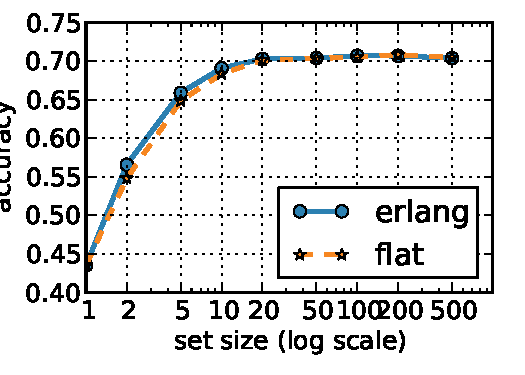
\includegraphics[width=0.45\textwidth]{figs/taskadaptation/diffprior_accuracy.pdf}
        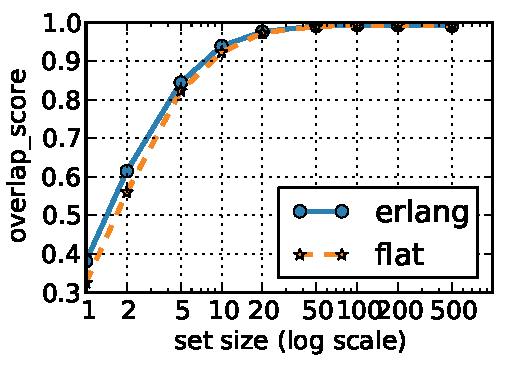
\includegraphics[width=0.45\textwidth]{figs/taskadaptation/diffprior_overlap_score.pdf}
    \caption{Performance comparison between using the ground-truth prior (erlang) and using the uninformed prior (flat). The top figure shows accuracy and the bottom figure shows the overlap score.}\label{fig:adapt:prior}
\end{figure}


\subsection{Online Evaluation}\label{subsec:online}
Our final evaluation tests the performance of the proposed method in an online fashion - when images of an unknown task come as a streaming sequence. Intuitively, our algorithm obtains better information about the unknown task as new images arrive, which would in turn increase the classification accuracy. We test such conjecture by evaluating the averaged accuracy of the $n$-th image, over multiple independent test query sequences that are generated in the same way as described in the previous subsection.

Figure \ref{fig:online} shows the average accuracy of the $n$-th query image, as well as the overlap between the identified task so far and the ground truth task. With the joint probabilistic inference, we obtain a significant performance increase after only a few images. This has particular practical interest, as one may want the computer to quickly adapt to a new task / environment with only a small number of queries. It is worth pointing out that with heuristic task estimation methods (see the baselines in Figure \ref{fig:online} left), one may incorrectly assert the latent task, which then hurts classification performance for the first few query images.

\begin{figure}
    \centering
    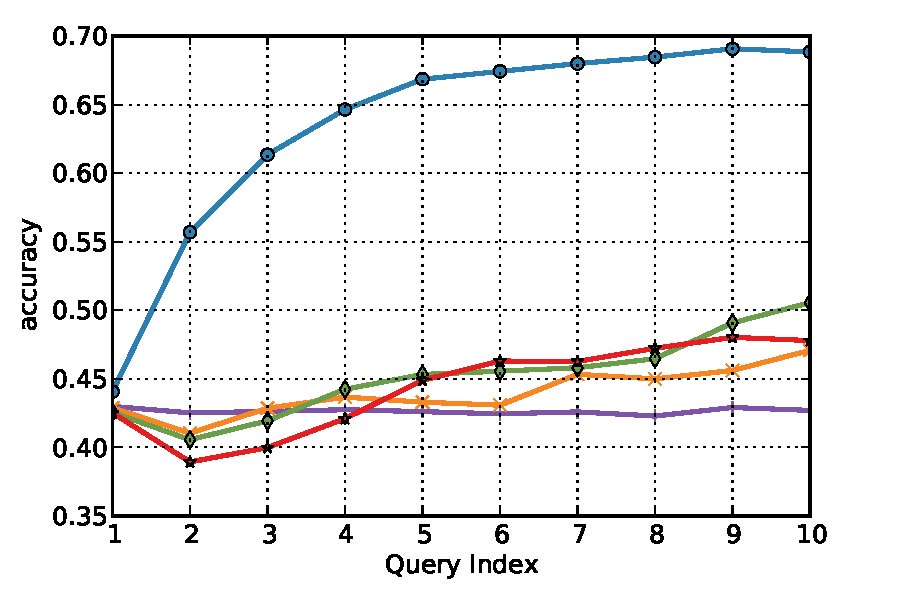
\includegraphics[width=0.45\textwidth]{figs/taskadaptation/online_accuracy.pdf}%
    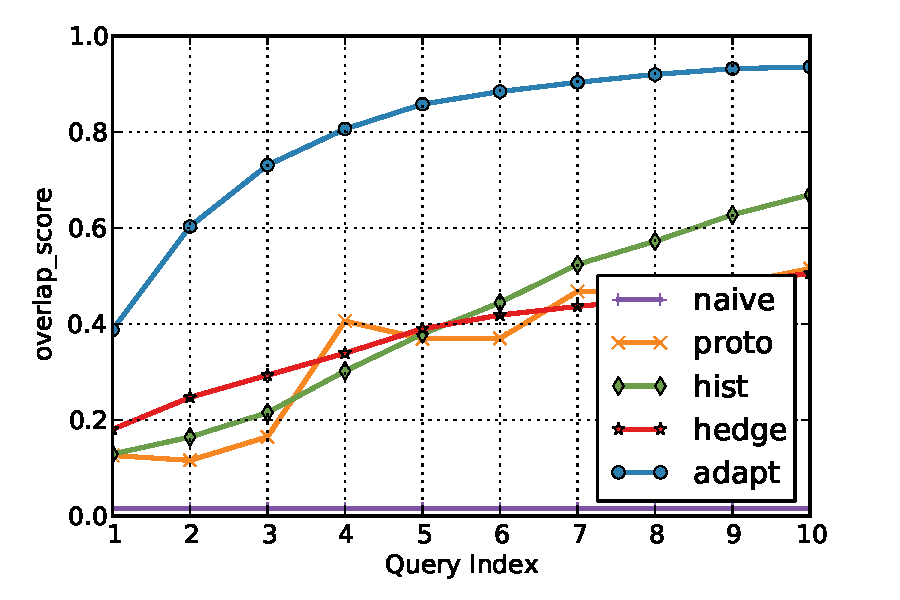
\includegraphics[width=0.45\textwidth]{figs/taskadaptation/online_overlap_score.pdf}
    \caption{Classification accuracy (left) and task overlap score (right) of our online algorithm against baselines. See subsection \ref{subsec:online} for details.}\label{fig:online}
\end{figure}

\section{Summary}
This chapter provides a concise example on how interdisciplinary research combining vision and cognitive science would allow smarter vision systems to be learned. We focused on a problem - latent task adaptation - that commonly appears in real-world applications but have little existing research on, and showed that an efficient, concept learning inspired framework is able to both discover the latent task context and better predict the categories under the specific task.

\section*{Notes}
Parts of this chapter have appeared in peer-reviewed publications as we list below:
\begin{enumerate}
\item Yangqing Jia, Trevor Darrell. Latent Task Adaptation with Large-scale Hierarchies. ICCV 2013.
\end{enumerate}